% Appendix A

\chapter{Mathematical Tools: Near Wall Modelling} % Main appendix title

\label{AppendixB} % For referencing this appendix elsewhere, use \ref{AppendixA}

\lhead{Appendix B. \emph{Mathematical Tools: NWM}} % This is for the header on each page - perhaps a shortened title

\section{Stress boundary conditions}\label{stresseq}
The viscous term in the weak form of NS equation in Equation~\ref{weak1} can be expanded using \textit{Integration by Parts} as follows
\begin{equation}
\left(\nu \nabla^{2} \pmb{u}, \pmb{v}\right) = \left(2\nu \nabla \nabla^{s} \pmb{u}, \pmb{v}\right) = 2\nu\int_{\Omega}  \nabla \nabla^{s} \pmb{u} \cdot \pmb{v} \mathrm{d}^{3}\pmb{x} = -  2\nu\int_{\Omega}  \nabla^{s} \pmb{u} \cdot \nabla^{s} \pmb{v} \mathrm{d}^{3}\pmb{x} + \int_{\Omega} 2\nu \nabla \left(\nabla^{s} \pmb{u} \cdot \pmb{v}\right) \mathrm{d}^3\pmb{x}
\end{equation}

$\nabla^{s}$ is the symmetric part of the gradient tensor given as $\frac{1}{2}\left(\nabla () + \nabla ()^{T}\right)$ and fluid stress in $\Omega$ is $\sigma_{ij} - \frac{1}{3}\sigma_{kk}\delta_{ij} = -2\nu \nabla^{s} \pmb{u}$ (Newton's linear stress-strain rate relation)

$$\nabla^{2} \pmb{u} = 2\nabla \nabla^s \pmb{u}$$ from the divergence constraint $\nabla \cdot \pmb{u} = 0$. \\
From Gauss divergence theorem: volume integral $\Omega$ $\rightarrow$ surface integral $\partial \Omega$
\begin{equation}
\int_{\Omega}2\nu \nabla \left(\nabla^{s} \pmb{u} \cdot \pmb{v}\right) \mathrm{d}^3\pmb{x} =  \oint_{\partial \Omega} 2\nu \nabla^{s} \pmb{u} \cdot \pmb{n} \pmb{v} \mathrm{d}S
\end{equation}


where $\pmb{n}$ is the outward unit normal on the surface $\partial \Omega$.\\

Closure of $2\nu \nabla^{s}  \pmb{u}$ in $\partial \Omega$ : \textit{ Wall Shear Stress}.
\begin{equation}
\boxed{\oint_{\partial \Omega} 2\nu \nabla^{s} \pmb{u} \cdot \pmb{n} \pmb{v} \mathrm{d}S = \oint_{\partial \Omega} \tau_{w}^{model} \cdot \pmb{n} \pmb{v} \mathrm{d}S}
\end{equation}
 

The functional space for $\pmb{u}$ (velocity) for such boundary conditions have to be relaxed from $H_0^1(\Omega)^3$ to $H^1(\Omega)^3$ (See Appendix~\ref{galproj}). For stress-free boundary conditions, the obvious outcome is $\nabla^{s} \pmb{u} = 0$.


\section{Elemental Level Filtering}\label{elfilt}
For the explicit filtering approach in near-wall modelling we use the modal approach of Boyd~\cite{boyd3}, see also~\cite{black}, \cite{bouf}. With the modal filtering technique, decomposition of the variable $u$ into the modal basis is sought,
\begin{equation}
u(\xi_i) = \sum_{k=0}^N{\hat{u}_k\phi_k(\xi_i)},\label{eq:modal}
\end{equation}
where $\xi_i, i = 0, \cdots, N$ represent the GLL clustering of the nodes, and the modal basis $\{\phi\}$,
\begin{equation}
\phi_0 = L_0(\xi),\ \ \phi_1 = L_1(\xi) \ \ \ \mbox{and}\ \ \ \ \phi_k = L_k(\xi) - L_{k-2}(\xi), \ \ \ 2\le k\le N  
\end{equation}
forms the hierarchical set of functions constructed from the Legendre polynomials $L_k(\xi)$. The bubble functions $\phi_k$,are designed to preserve homogeneous Dirichlet boundary conditions, since $\phi_k(\pm 1) = 0$ for $k\geq 2$ (See Appendix~\ref{legpol} for details). The inhomogeneous Dirichlet boundary conditions are satisfied by the low order polynomials $\phi_0, \phi_1$. The mapping between the nodal Lagrangian basis and the modal representation defined by Eq.~(\ref{eq:modal}) can be cast into the matrix form\begin{equation}
\pmb{u} = \Phi \pmb{\hat{u}}.
\end{equation}
%The filtered function $\tilde{u}(\xi) = \sum_{k = 0}^{N}\sigma(k;N)\hat{u}_k\phi_k(\xi)$, with $\sigma$ being the filtered coefficient, in matrix-vector format are elegantly presented below as \\

\begin{figure}
\centering
        \begin{subfigure}[b]{0.32\textwidth}
                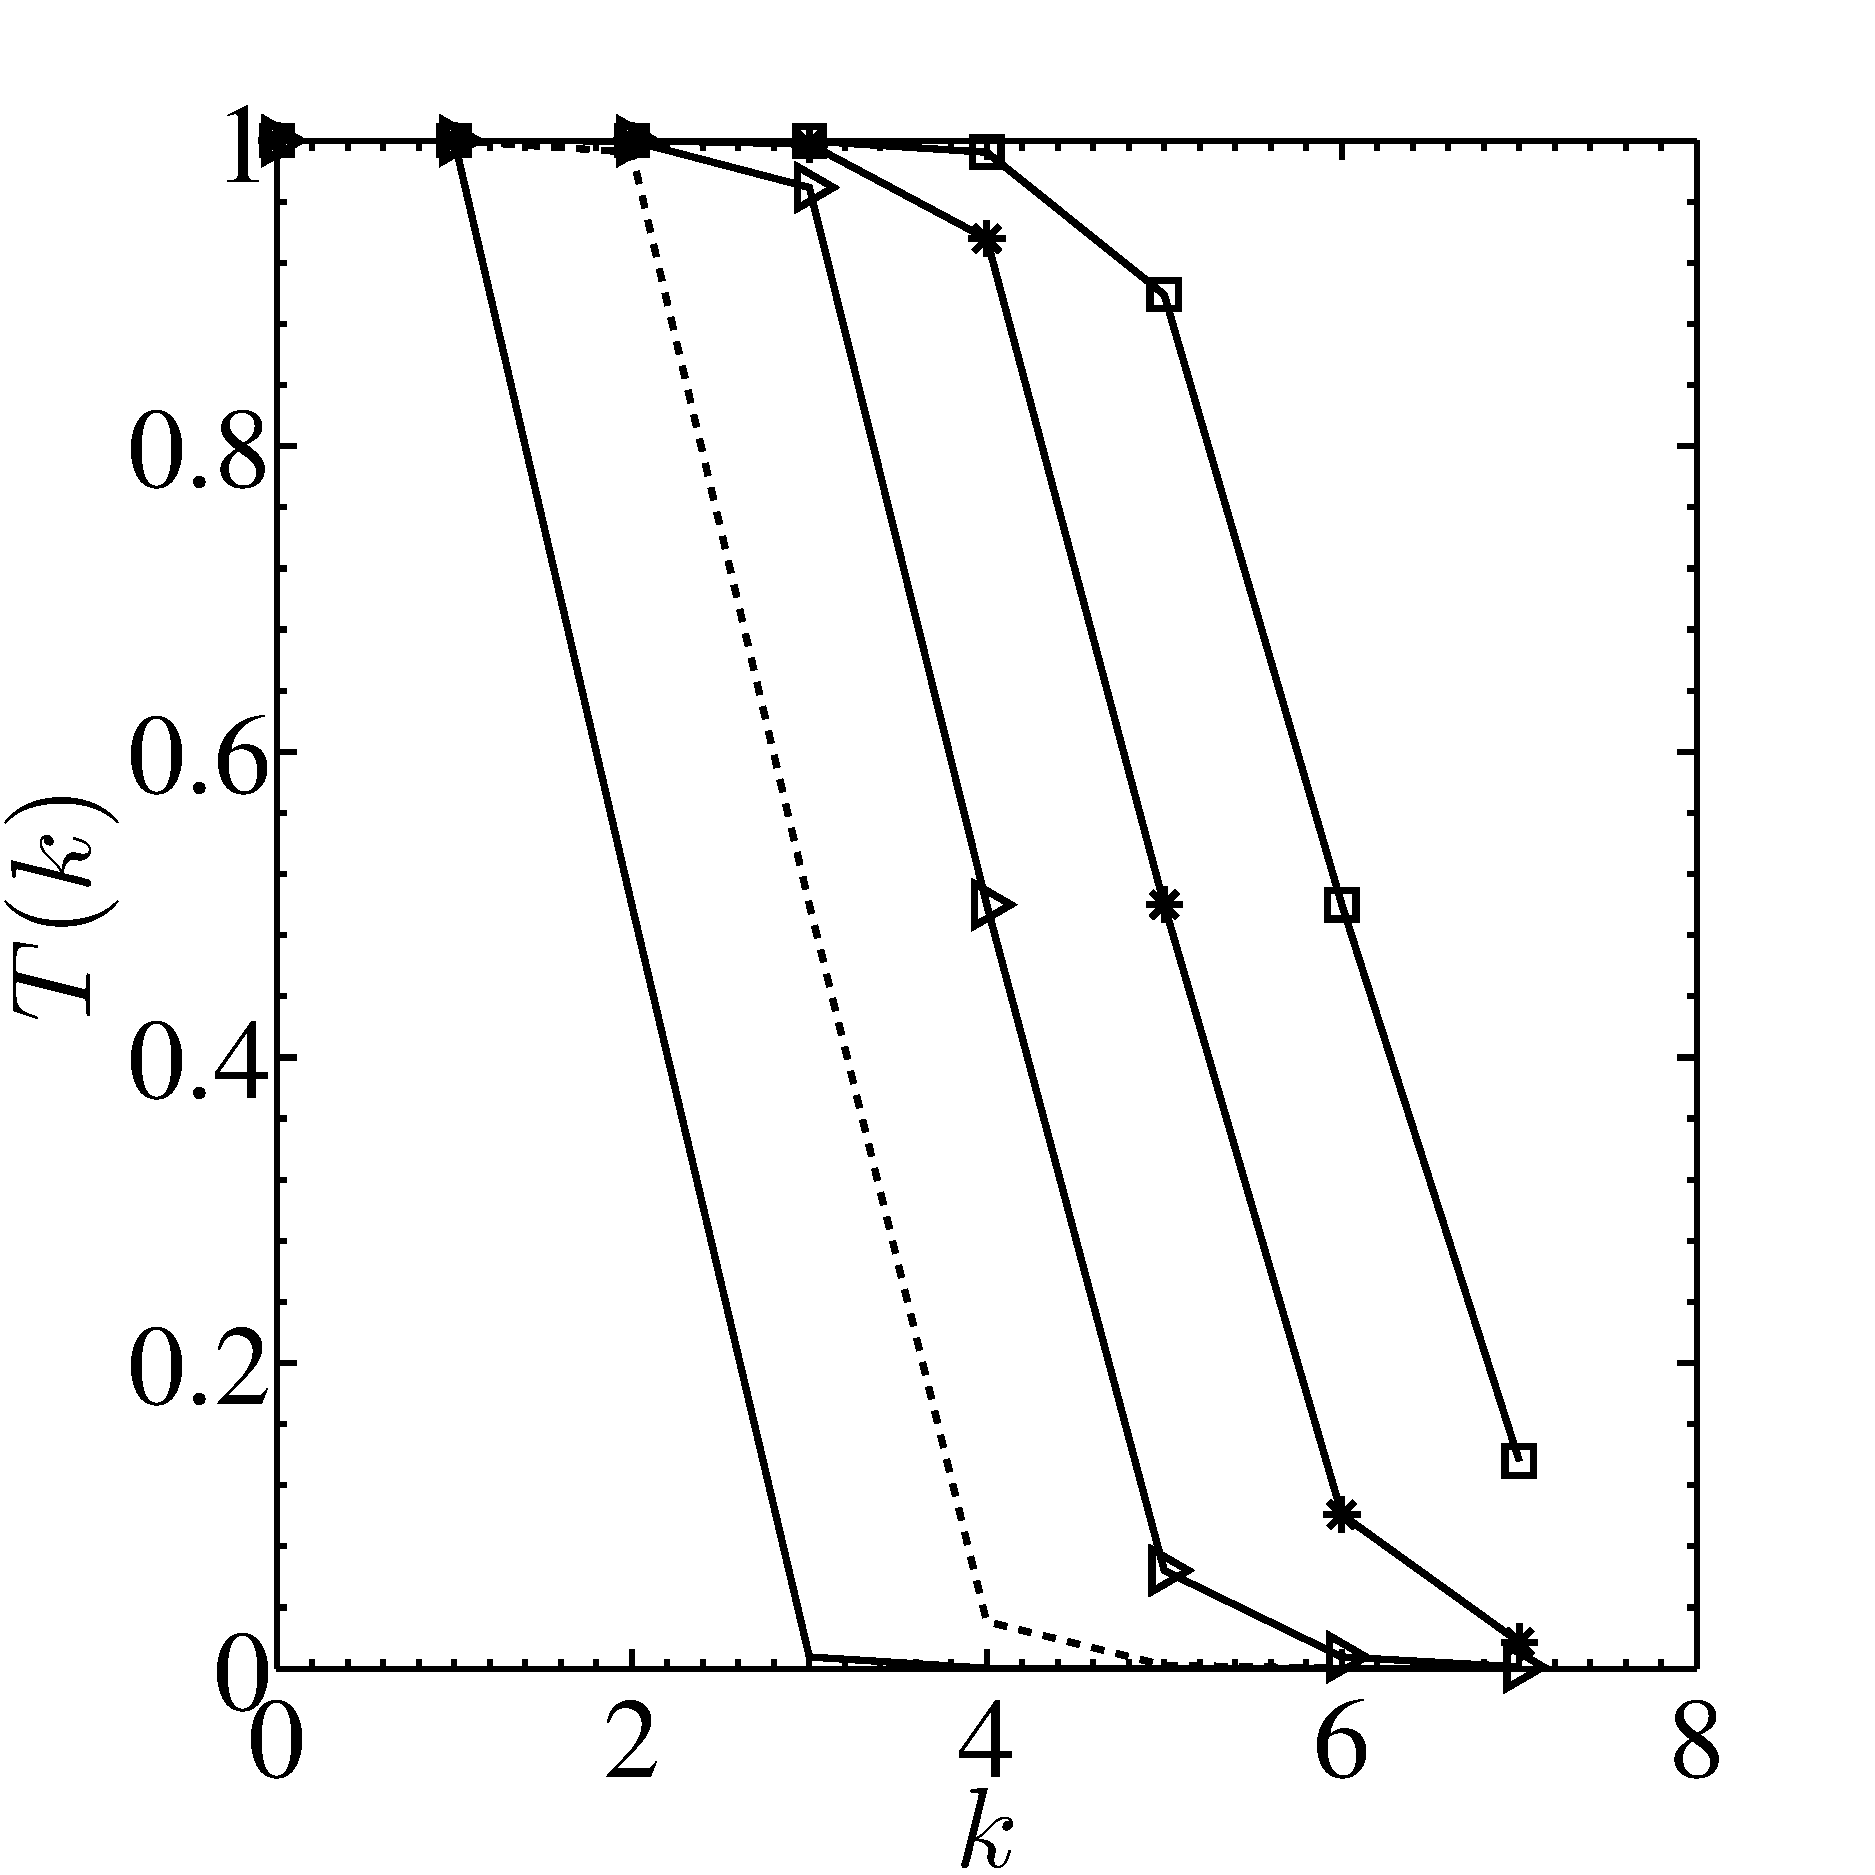
\includegraphics[width=\linewidth]{Figure/filter1.pdf}
                \caption{}
                \label{fig:filt1}
        \end{subfigure}%
          \begin{subfigure}[b]{0.32\textwidth}
         \centering
                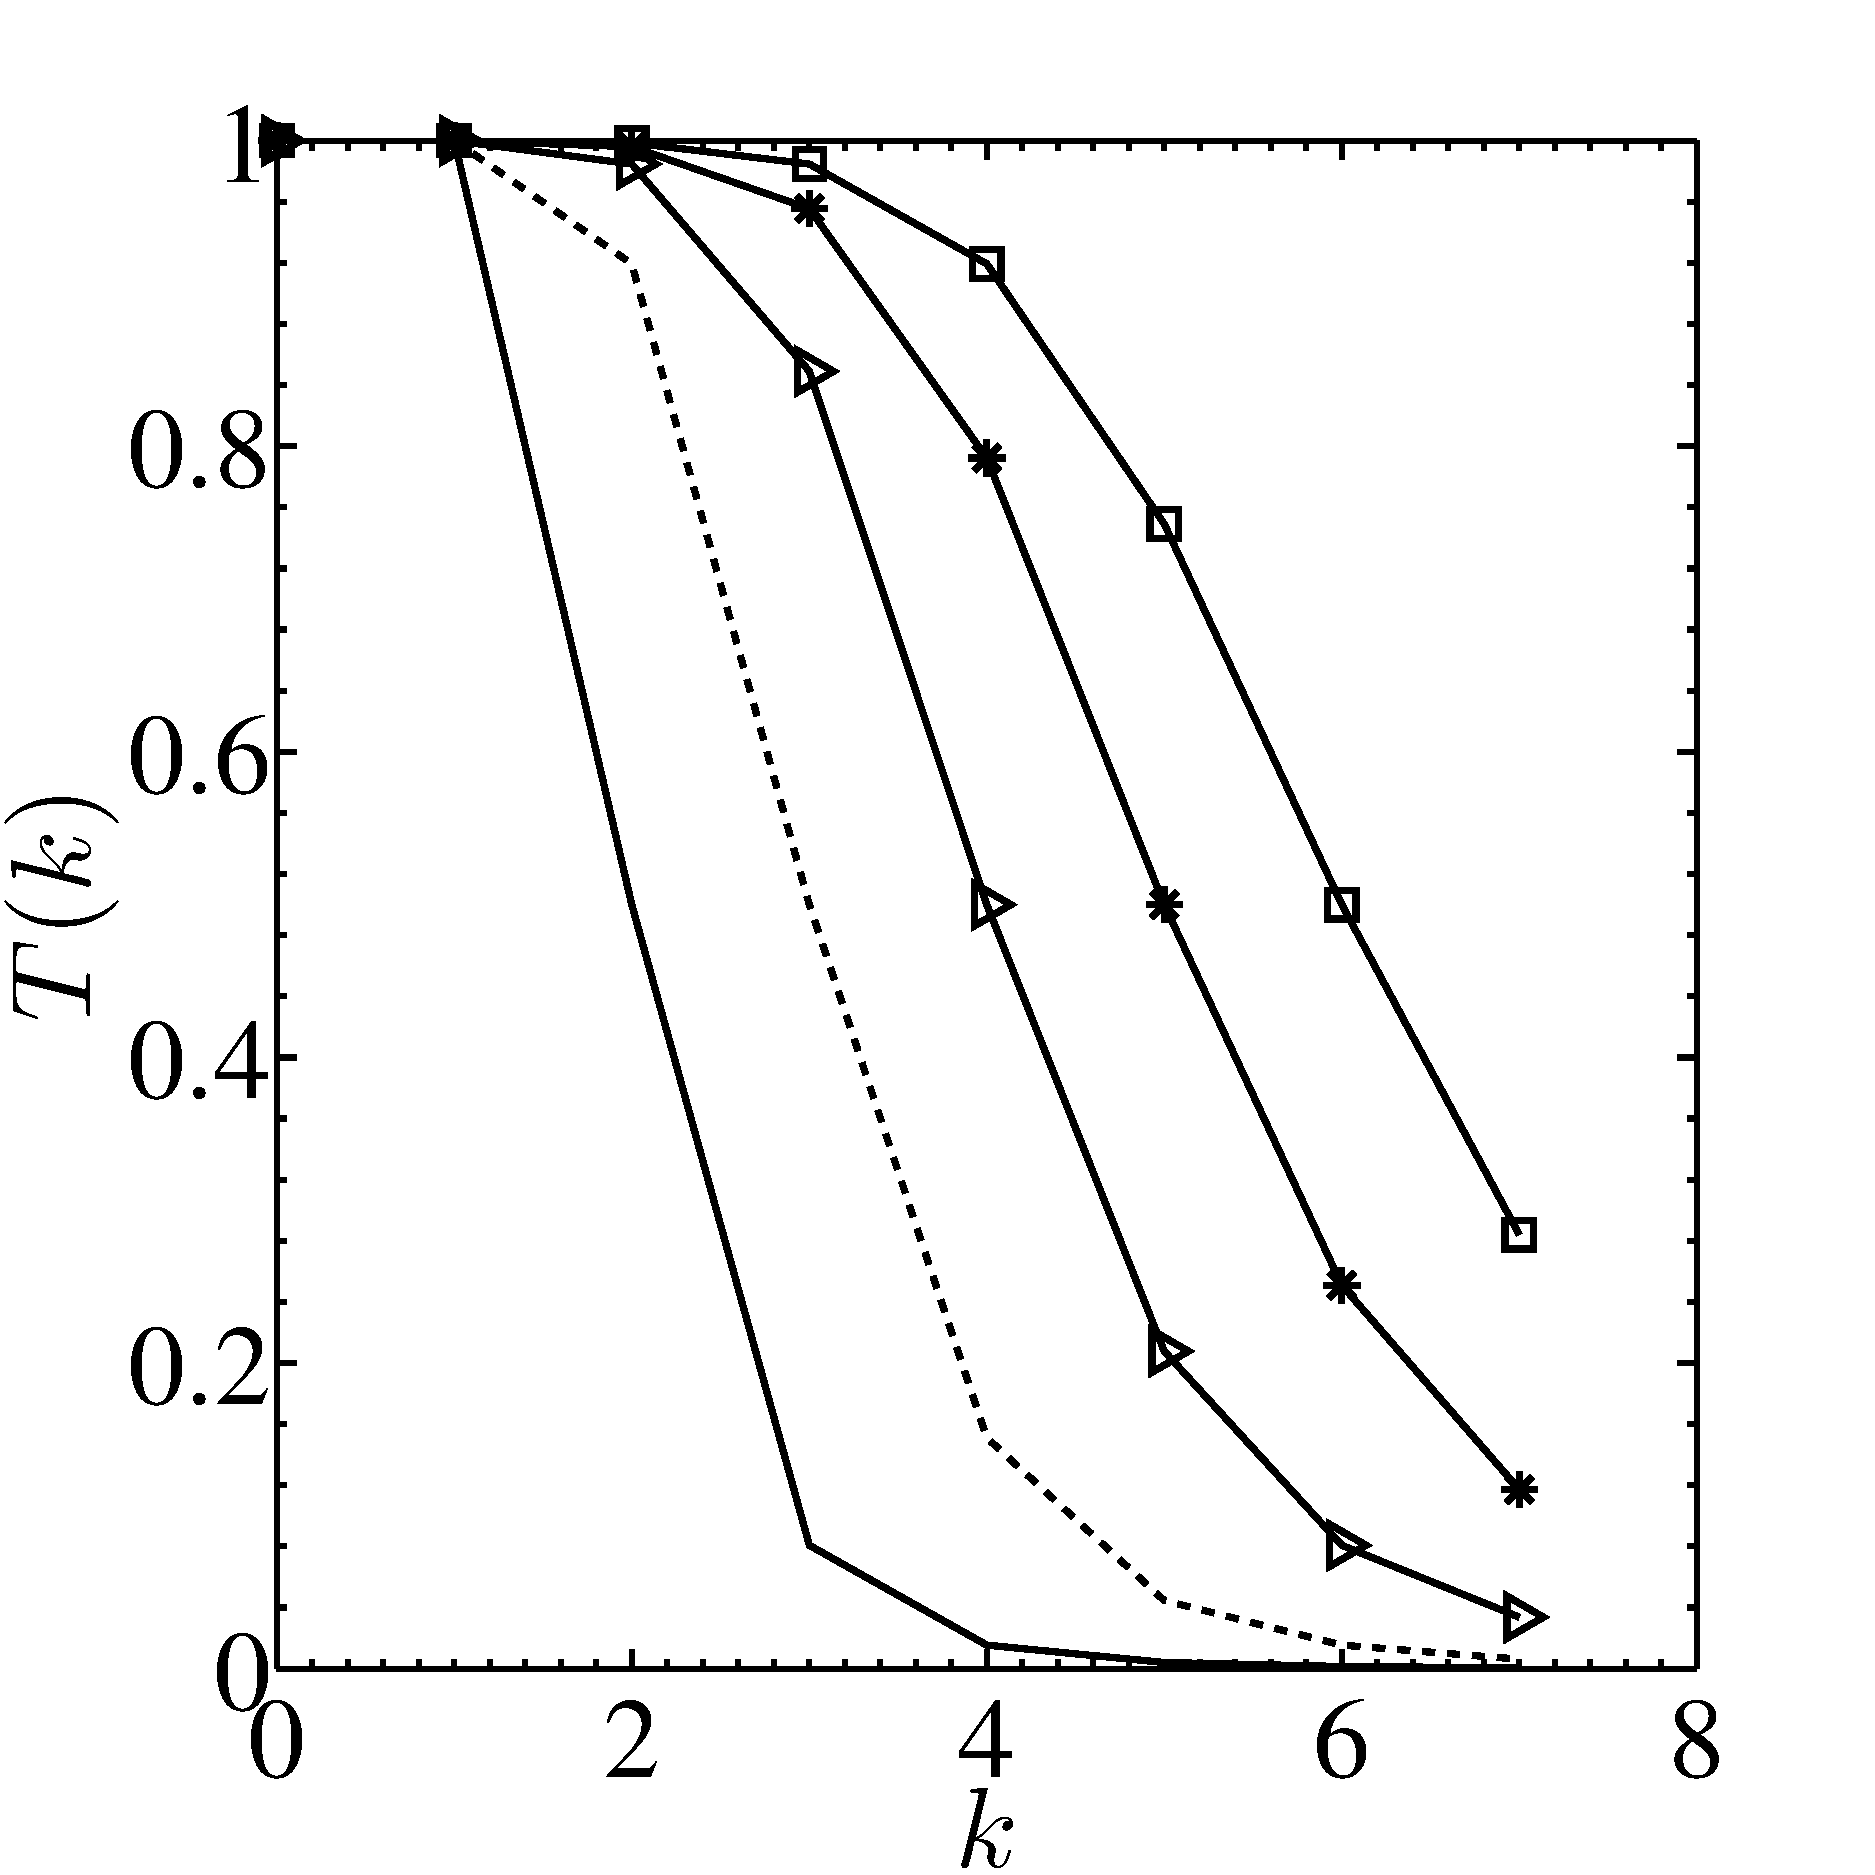
\includegraphics[width=\linewidth]{Figure/filter2.pdf}
                 \caption{}
                 \label{fig:filt2}
         \end{subfigure}%
         \begin{subfigure}[b]{0.32\textwidth}
         \centering
                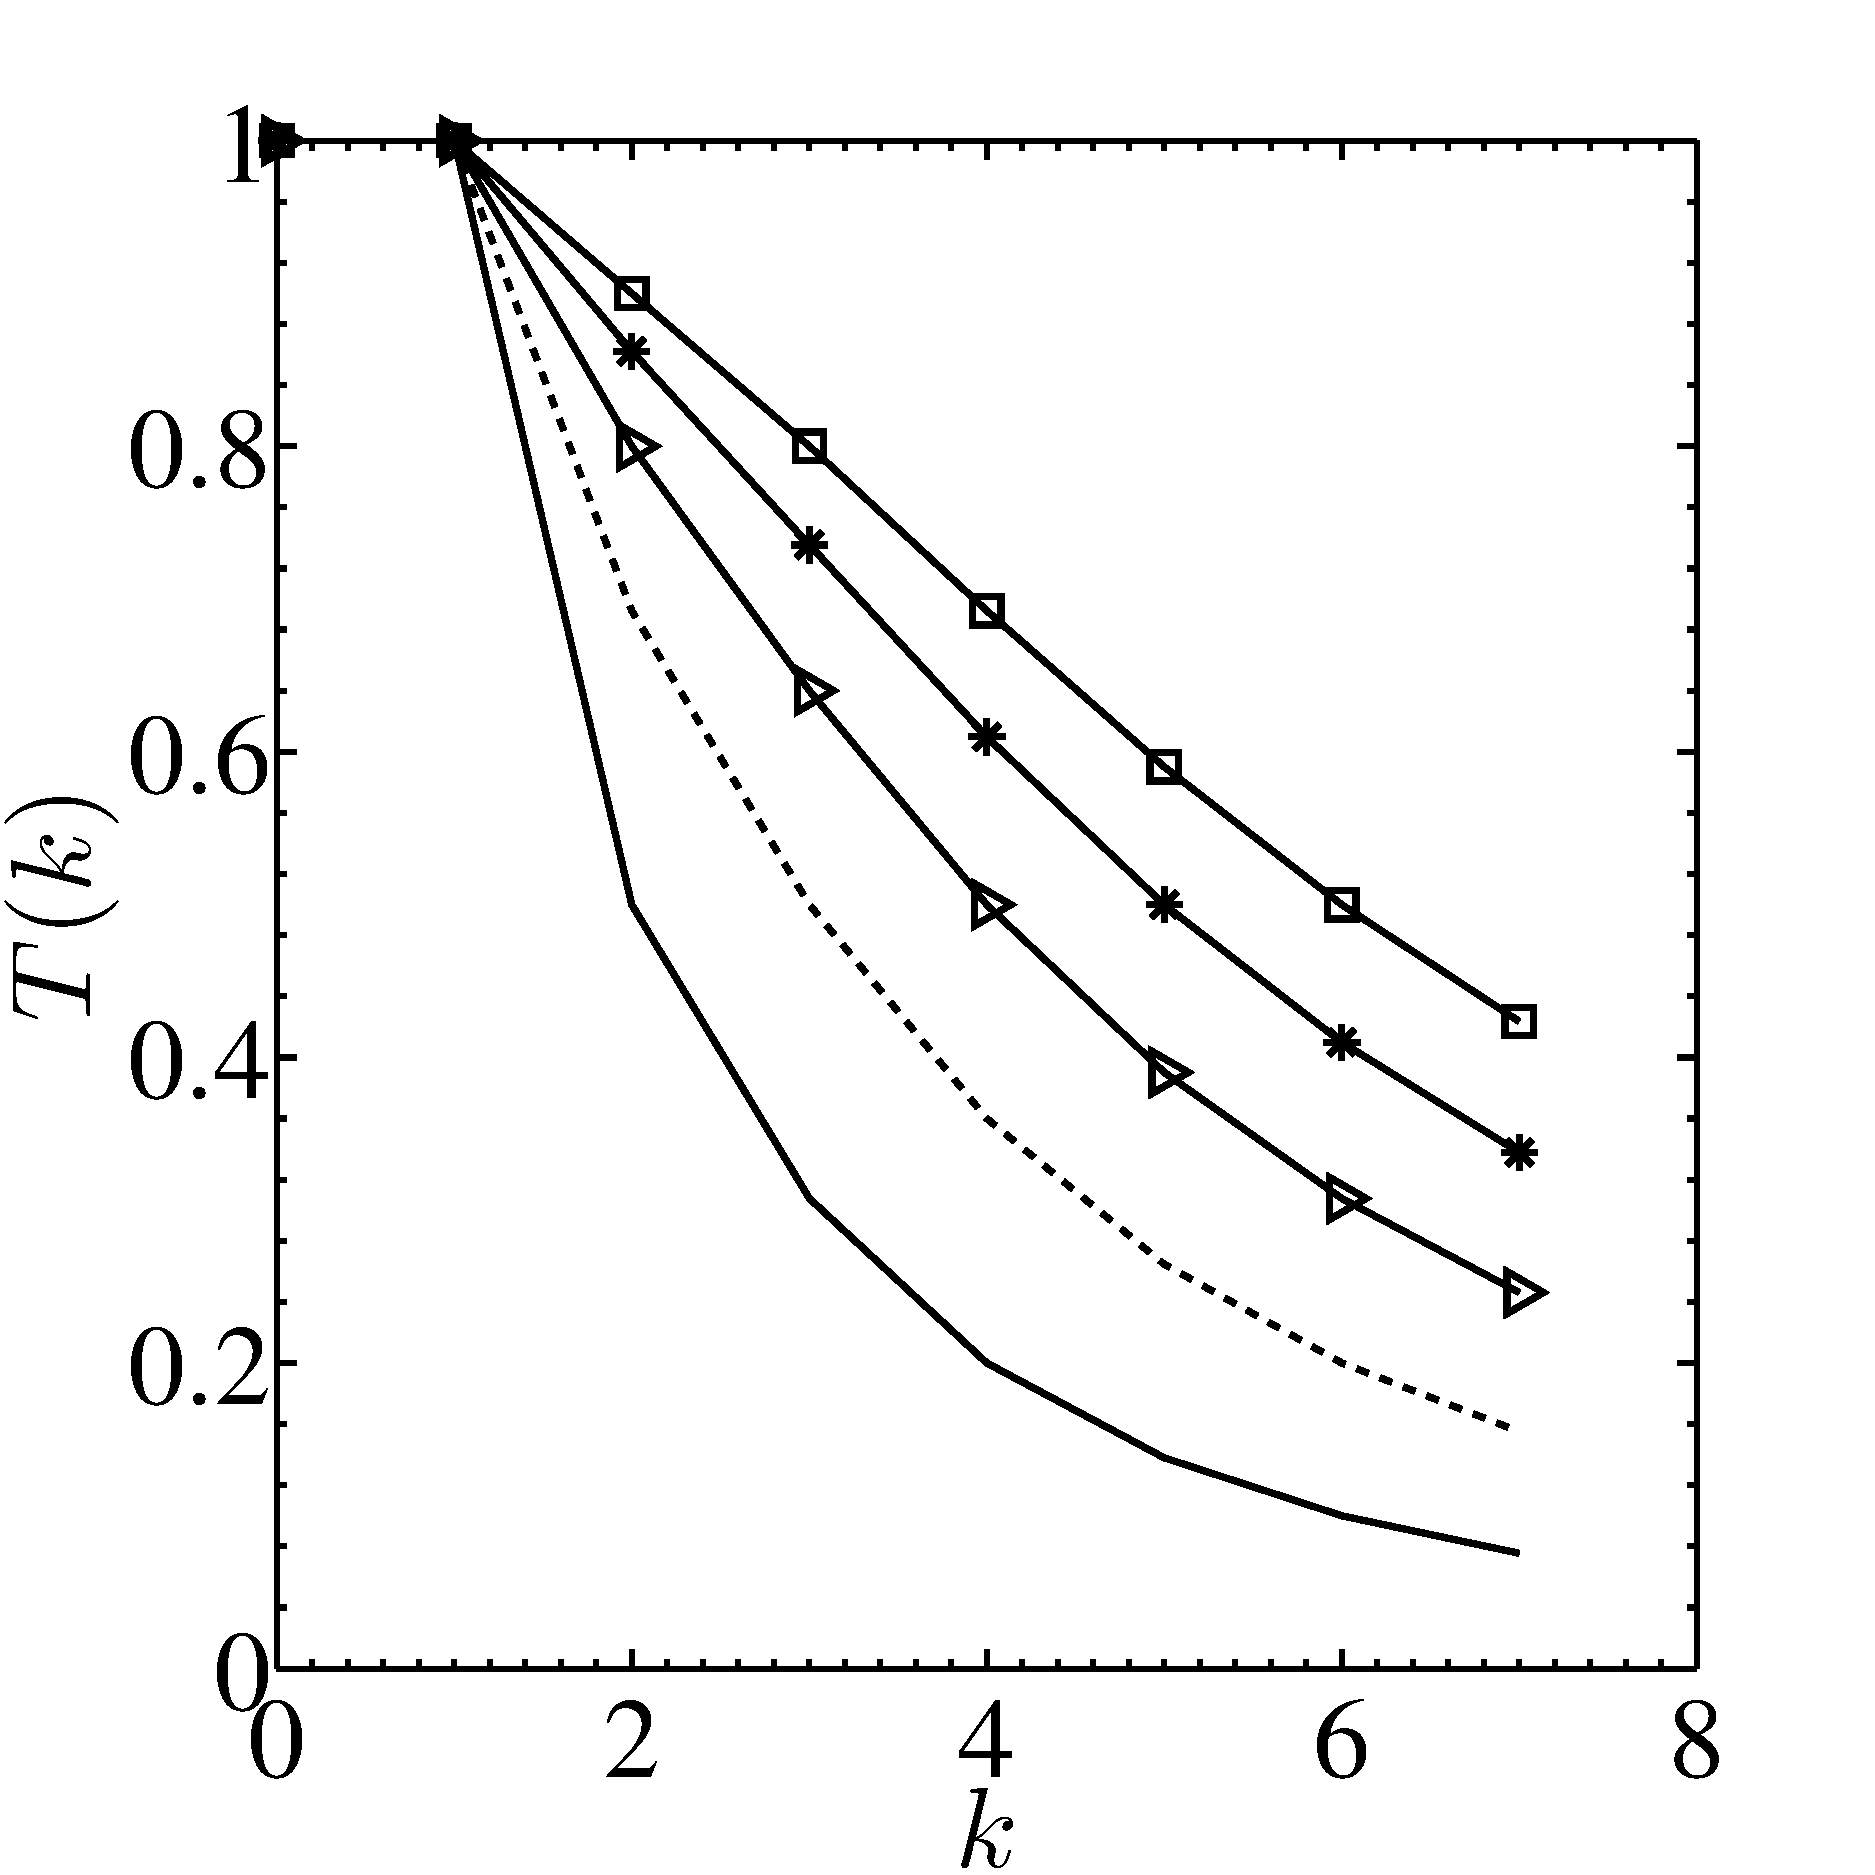
\includegraphics[width=\linewidth]{Figure/filter3.pdf}
                 \caption{}
                 \label{fig:filt3}
         \end{subfigure}
        \caption[Filter transfer function for different $(k_c, \ \gamma)$: Near Wall Modelling]{Filter transfer function ${T}(k) = (1 + (k/k_{c})^\gamma)^{-1}$ (a) $\gamma = 12$ (b) $\gamma = 6$ (c) $\gamma = 2$.\hspace{2mm} $-$, $k_c = 2$; $--$, $k_c = 3$; $-.- \triangle$ $k_c = 4$; $-\star$, $k_c = 5$; $- \Box$ $k_c = 6$ $|$ ${T}(k_c) = \frac{1}{2}$. The total number of modes $k_{max} = N =7$, corresponding to GLL nodes = 8 (used in our simulation)}\label{fig:elem_filter}
\end{figure}

The low-pass filtering is performed in the modal space through a diagonal matrix $\mathbb{T}$ whose components are $T_0 = T_1 = 1$ (satisfying $C_0$ inter-element continuity) and $T_k = f(k;k_c) = 1/(1 + (k/k_c)^\gamma) , \ \ \ 2\le k\le N$. $f(k;k_c$) is an attenuation function with increasing higher mode $k$, and $k_c$ is the cut-off value such that $T_k|_{k=k_c} = 1/2$ (See Figure~\ref{fig:elem_filter}). Both parameters  $k_c$ and $\gamma$, determine the precise shape of the filter transfer function. Decreasing $k_c$ quite straightforwardly attenuate the large scale contents of the filtered velocity $\widetilde{u}_{i}$, while decreasing $\gamma$ smoothens the transfer function more towards non-projective filtering as seen in Figure~\ref{fig:filt1},~\ref{fig:filt2},~\ref{fig:filt3}. 
 The filtering process in one dimension is given by
\begin{equation}
\widetilde{\pmb{u}} = \mathcal{G}*\pmb{u} = \Phi\mathbb{T}\Phi^{-1}\pmb{u}.
\end{equation}
Extrapolation to 3D field can be achieved from 1D filter by a fast tensor product application~\cite{lynch}

